% D.25 切割线定理：AB 直径，PA 切于 A，割线 PCD（C 在 PD 间），PA=6，PC=4
\documentclass[tikz,border=4pt]{standalone}
\usepackage{ctex}
\usepackage{amsmath}
\usetikzlibrary{calc}
\begin{document}
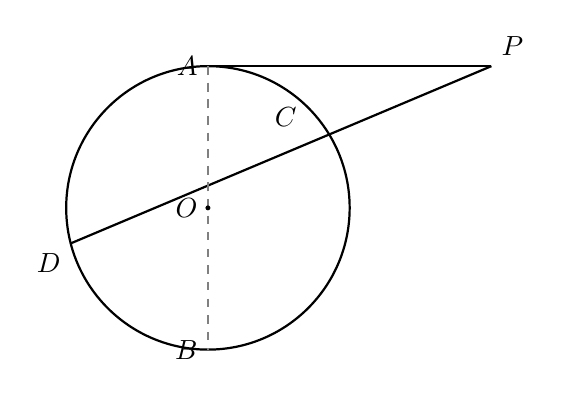
\begin{tikzpicture}[scale=0.6, thick]
  \coordinate (O) at (0, 0);
  \pgfmathsetmacro{\r}{3}
  \draw (O) circle (\r);
  \coordinate (A) at (0, \r);
  \coordinate (B) at (0,-\r);
  % P 在 A 上方切线（A 处切线水平）：PA=6 → P=(6, 3)
  \coordinate (P) at (6, 3);
  % 割线 PCD 过 P 交圆于 C、D：取直线斜率使得 PC=4
  % 简化：手工选直线 P->(-3,-0.5)；该直线与圆交两点
  \coordinate (D) at (-2.9, -0.75);
  \coordinate (C) at ( 1.2,  1.5);

  \draw (A) -- (P);
  \draw (P) -- (D);
  \draw[gray, dashed] (A) -- (B);
  \draw[gray, dashed] (O) -- (A);

  \fill (O) circle (1.5pt);
  \node[left]  at (O) {$O$};
  \node[left]  at (A) {$A$};
  \node[left]  at (B) {$B$};
  \node[above right] at (P) {$P$};
  \node[above right] at (C) {$C$};
  \node[below left]  at (D) {$D$};
\end{tikzpicture}
\end{document}
